% Bagian Hasil Percobaan
\section*{Hasil Percobaan} % Jika ada hasil percobaan

Hasil percobaan yang diperoleh adalah sebagai berikut:

\begin{enumerate}
    \item \textbf{Hasil Konfigurasi:} Untuk Tahapan Konfigurasi Awal, DHPC Server, dan Firewall dan NAT
    
    \begin{figure}[H]
        \centering
        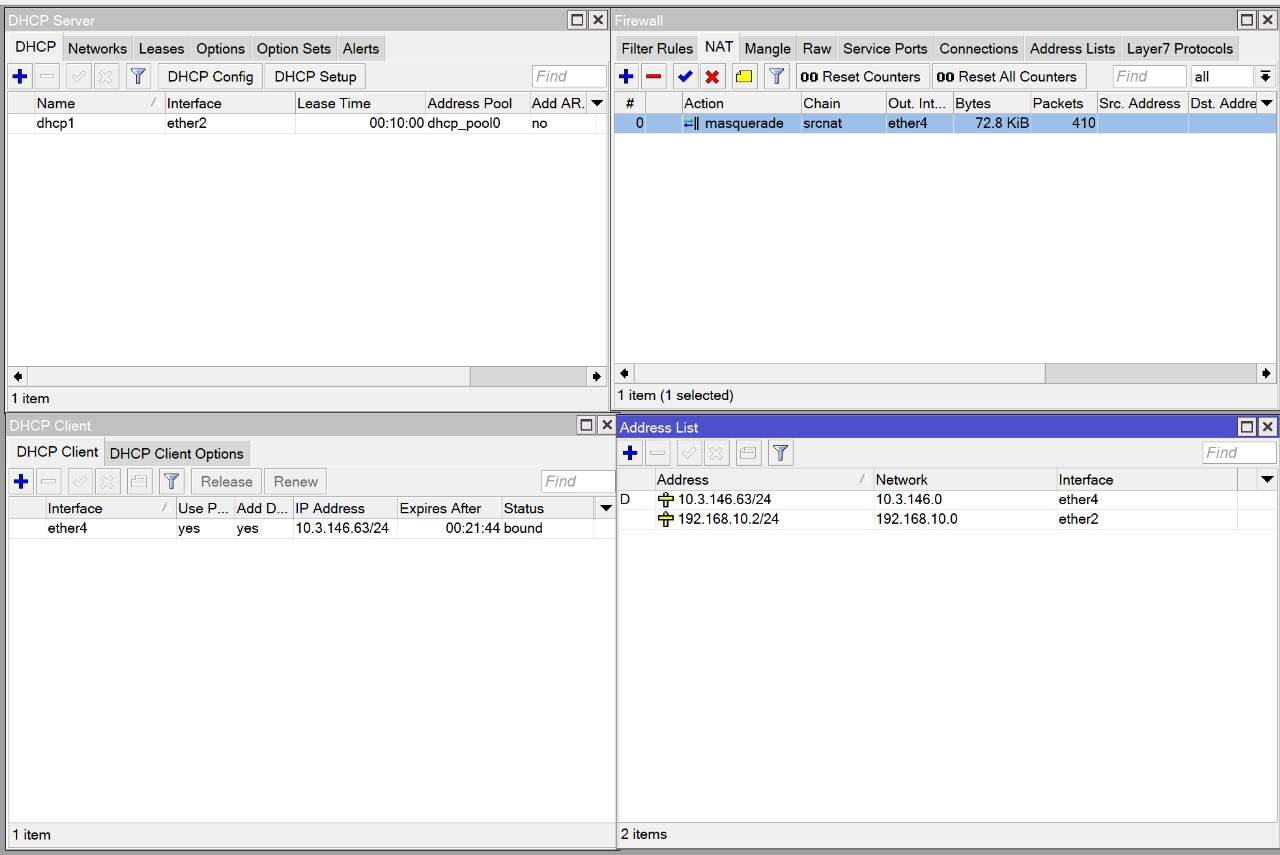
\includegraphics[width=0.9\textwidth]{img/Konfigurasi_Percobaan_1.jpeg}
        \caption{Konfigurasi Awal}
        \label{fig:konfigurasi_awal}
    \end{figure}

    \item \textbf{Pengujian Koneksi:} Koneksi ke jaringan publik berhasil diuji dengan melakukan cek bandwidth menggunakan speed test.
    
    \begin{figure}[H]
        \centering
        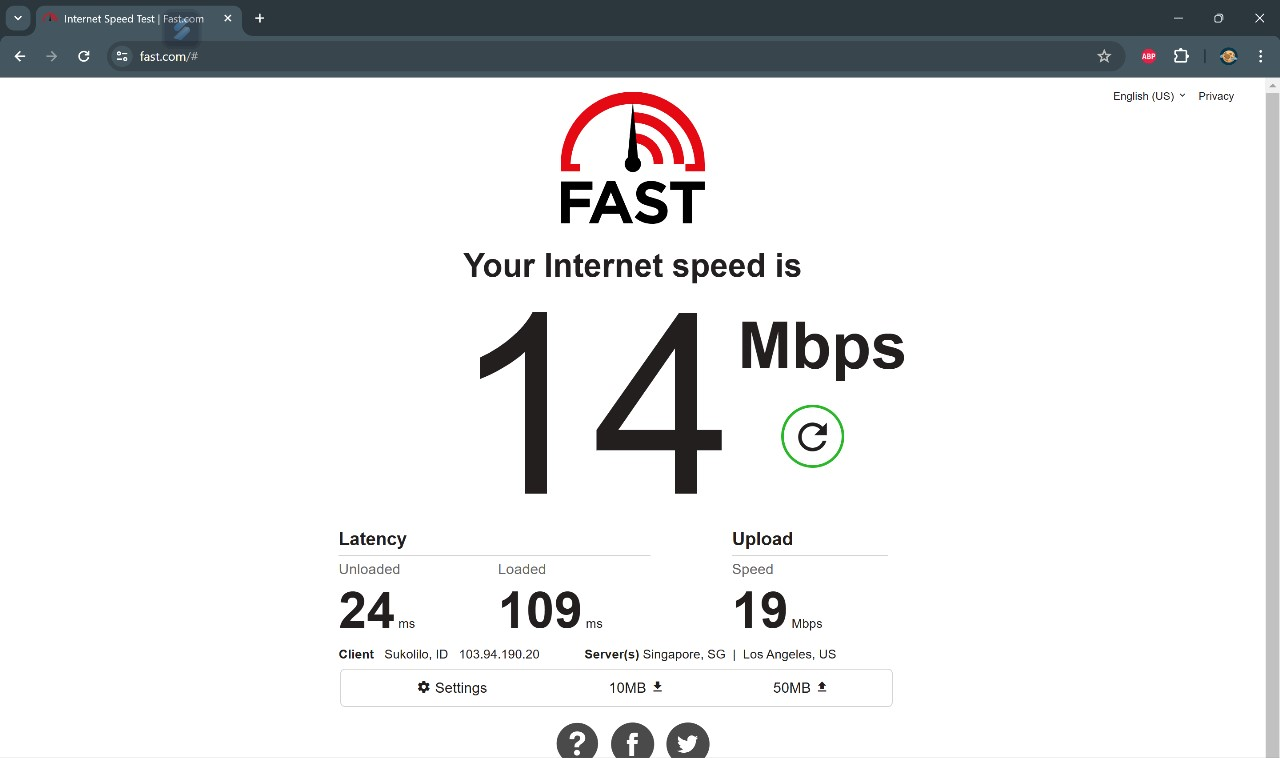
\includegraphics[width=0.7\textwidth]{img/Hasil Tanpa Pengaturan.jpeg}
        \caption{Pengujian Koneksi}
        \label{fig:pengujian_koneksi}
    \end{figure}

    \item \textbf{Pengujian Pembatasan Bandwidth:} Pembatasan bandwidth berhasil diuji dengan melakukan speed test setelah pembatasan bandwidth dilakukan. Dengan konfigurasi seperti pada Gambar \ref{fig:konfigurasi_bandwidth}, hasil pengujian seperti pada Gambar \ref{fig:pengujian_bandwidth}.
    
    \begin{figure}[H]
        \centering
        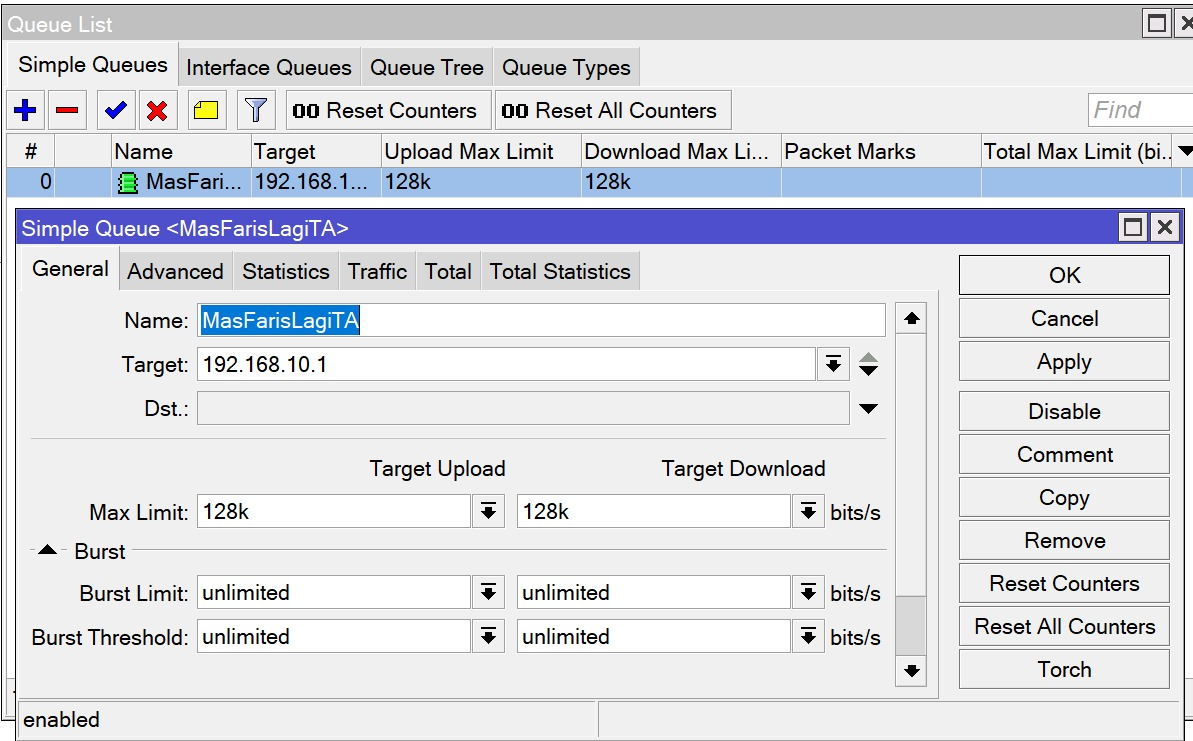
\includegraphics[width=0.7\textwidth]{img/Set Pertama.jpeg}
        \caption{Konfigurasi Pembatasan Bandwidth}
        \label{fig:konfigurasi_bandwidth}
    \end{figure}

    \begin{figure}[H]
        \centering
        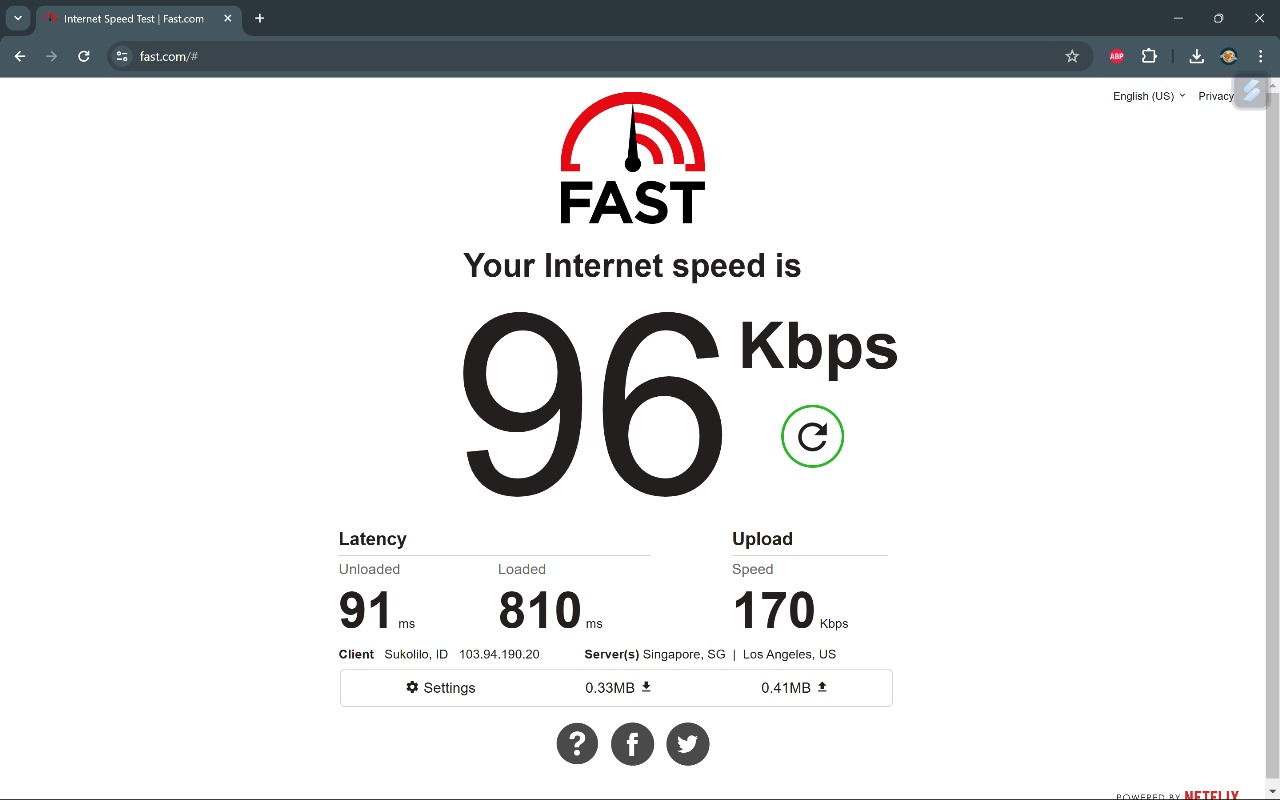
\includegraphics[width=0.7\textwidth]{img/Hasil Set pErtama.jpeg}
        \caption{Pengujian Pembatasan Bandwidth}
        \label{fig:pengujian_bandwidth}
    \end{figure}

    \item \textbf{Konfigurasi Pembatasan Bandwidth Pada 2 Client:} Pembatasan bandwidth pada 2 client berhasil diuji dengan melakukan konfigurasi pembatasan bandwidth. Dengan konfigurasi PC 1 dan PC 2 seperti pada Gambar \ref{fig:konfigurasi_client_1}.
    
    \begin{figure}[H]
        \centering
        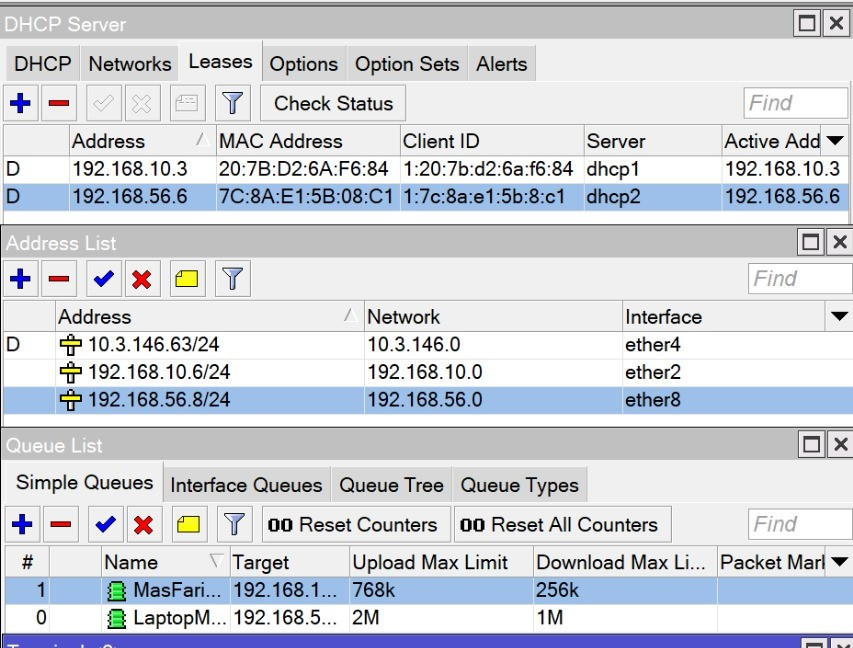
\includegraphics[width=0.7\textwidth]{img/Ngatur PC 2.jpeg}
        \caption{Konfigurasi Pembatasan Bandwidth PC 1}
        \label{fig:konfigurasi_client_1}
    \end{figure}

    \item \textbf{Pengujian Pembatasan Bandwidth Pada 2 Client:} Pembatasan bandwidth pada 2 client berhasil diuji dengan melakukan speed test setelah pembatasan bandwidth dilakukan. Dengan hasil pengujian seperti pada Gambar \ref{fig:pengujian_client_1} dan Gambar \ref{fig:pengujian_client_2}.
    
    \begin{figure}[H]
        \centering
        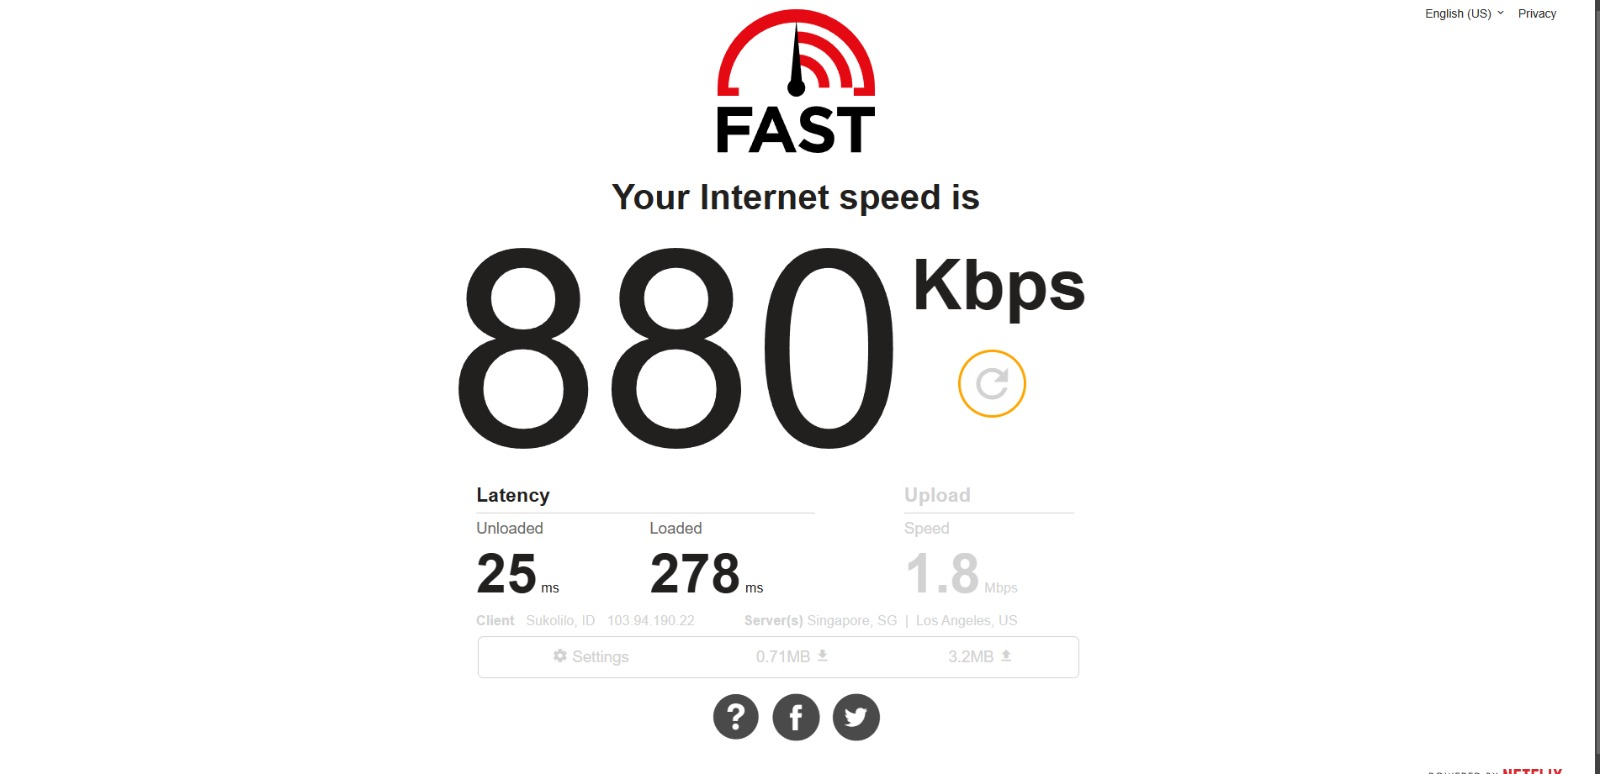
\includegraphics[width=0.7\textwidth]{img/Hasil PC 1.jpeg}
        \caption{Pengujian Pembatasan Bandwidth PC 1}
        \label{fig:pengujian_client_1}
    \end{figure}

    \begin{figure}[H]
        \centering
        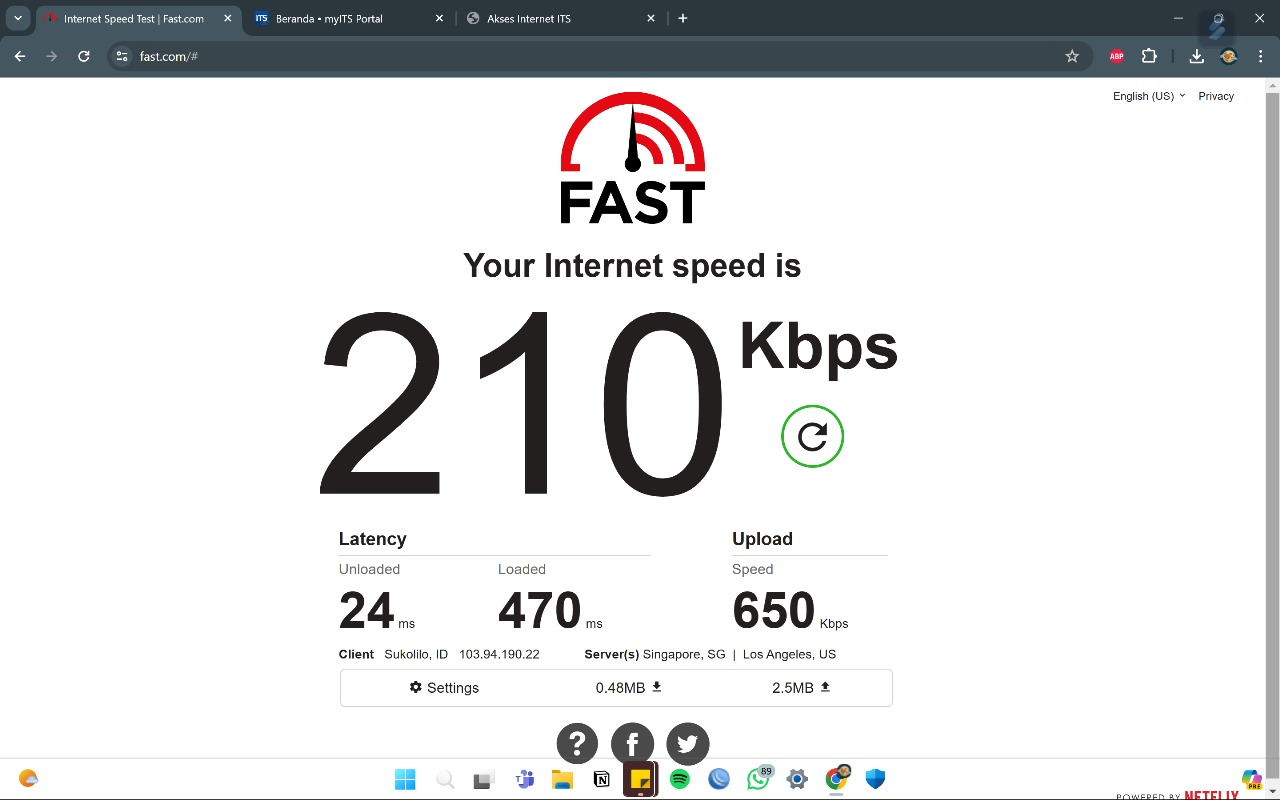
\includegraphics[width=0.7\textwidth]{img/Hasil PC 2.jpeg}
        \caption{Pengujian Pembatasan Bandwidth PC 2}
        \label{fig:pengujian_client_2}
    \end{figure}
    
\end{enumerate}